\documentclass{sig-alternate}


\usepackage{graphicx}

\newcounter{theorems}
\newtheorem{theorem}[theorems]{Theorem}

\begin{document}


\title{Probablistic Association Discovery using Functions of
  Observation Graph} 
\numberofauthors{2}

\author{
  \alignauthor 
  Hesen Peng \\
  \affaddr{Independent}\\
  \affaddr{136 102nd Ave SE Apt 326}\\
  \affaddr{Bellevue, Washington, USA 98004}\\
  \email{hesen.peng@gmail.com}  
  \alignauthor
  Tianwei Yu\\
  \affaddr{Dept of Biostatistics and Bioinformatics}\\
  \affaddr{Emory University}\\
  \affaddr{1518 Clifton Rd NE 3F}\\
  \affaddr{Atlanta Georgia, USA 30322}\\
  \email{tianwei.yu@emory.edu}
}

\date{\today{}}

\maketitle
 

\begin{abstract}
  Probablistic association discovery aims to identify the association
  between random vectors of their association, regardless of number of
  variables involved or linear/nonlinear functional forms. Application
  to high-dimensional data analysis has generated rising interest in
  probablistic association discovery.

  We developed a framework for probablistic association discovery on
  the Euclidean space using functions on the observation graph. We
  first discuss the property of mean observation distance and its
  novel application to association discovery. Then we generalize the
  advantageous property to a group of functions on the observation
  graph. The group of functions encapsulates major existing methods in
  association discovery, like mutual information and Mira score. We
  conducted numerical comparison that shows differentiated testing
  power under multiple scenarios. 

\end{abstract}


\category{H.4}{Information Systems Applications}{Miscellaneous}
\category{D.2.8}{Software Engineering}{Metrics}[complexity measures, performance measures]

\terms{Theory, Happy}

\keywords{ACM proceedings, \LaTeX, text tagging}


\section{Introduction}
\label{sec:intro}

In this paper we would like to propose and generalize new methods to
discover probablistic association between random vectors. Consider two
random vectors $X$ and $Y$ and $n$ pairs of independent and
indentically distributed (i.i.d.) random samples $\{X_i,
Y_i\}_{i=1}^n$. We would like to draw inference for the existence of
probablistic association between $X$ and $Y$ based on the $n$ pairs of
samples. The discussion in this paper will focus on the probablistic
association between continuous random variables defined in the
Euclidean space. However, general theory developed in this paper can
be applied in other spaces as well.

Classical association statistics like Pearson's correlation
coefficient assume functional forms (for example, piecewise linear,
monotonicity) between $X$ and $Y$, which are judged as
\emph{correlated} if
\begin{displaymath}
  Corr(X,Y) \ne 0
\end{displaymath}
Probablistic association statistic, as the name suggests, perceives
associations from the level of probablistic dependence. That is, $X$
and $Y$ are judged as independent if and only if their joint
probability density function can be factored
\begin{equation}
  \label{eq:independence}
  F(X,Y)= F(X) F(Y)
\end{equation}
where $F(\cdot)$ is the probability density function for the random
vector under consideration. Probabblistic association encapsulates a
larger group of associations than traditional correlation coefficient.
For example, probablistic association would consider nonlinear
interactions involving multiple variables.

We have noticed that multiple methods on probablistic association
discovery are linked to functions on the observation distance graph.
The distance graph consists of nodes representing each observation
$(X_i, Y_i)$ in the $p+q$ Euclidean space. Here $p$ and $q$ are the
dimensions of $X$ and $Y$, respectively. Edges of the observation
graph would connect two nodes (observations) if specific criteria is
satisfied.

For example, mutual information and its derivatives have been the most
popular probablistic association statistic to
date\cite{cite:my-cas-work, citation:MINE-science,
  tostevin2009mutual}. To estimate mutual information, the joint
entropy can be approximated using log-transformed $K$-nearest
neighbour distance averaged for each observation
\cite{PhysRevE.69.066138, leonenko2008,
  doi:10.1080/104852504200026815}.

Recent breakthrough on distance covariate \cite{székely2009,
  székely2007} sheds light on universal association discovery with
its simplicity of form and theoretical flexibility. Brownian distance
\cite{székely2009} covariate proposed \texttt{dCov} as
\begin{equation*}
  V_N^2 = \frac{1}{n^2}\sum_{k,l=1}^n D^{X}_{kl}D^{Y}_{kl}
\end{equation*}
where $D^{X}_{kl}$ and $D^{Y}_{kl}$ are linear functions of pairwise
distances between sample elements calculated with $X$ and $Y$
dimensions, respectively. Given fixed marginal distribution for $X$
and $Y$, large Brownian distance covariate suggests the existence of
probablistic association.

In an independent research, the authors proposed Mira score
\cite{my-dissertation} as
\begin{equation*}
  M = \sum_{k,l = 1}^n D^{(X,Y)}_{kl} w_{kl}
\end{equation*}
where $D^{(X,Y)}_{kl}$ is the distance between sample elements
calculated using both $X$ and $Y$ dimensions, and $w_{kl}=1$ when the
involved elements are nearest neighbors, $w_{kl}=0$ otherwise. Given
fixed marginal distribution for $X$ and $Y$, small Mira score suggests
the existence of probablistic association. 

We would like to discuss the property of functions applied to the
distances of the observation graph. The discussion of the section
below is inspired by comparing mean observation distance between
dependent and independent random vectors of the same marginal
distribution. Our intution suggest that when two random vectors are
probablistically associated, their observation distances tend to be
smaller than their independent counterparts.

Take Figure \ref{fig:comparison} for example, both plots show 300
samples from two bivariate random vectors. Observations on the left
panel are sampled from independent bivariate normal distributions.
Observations on the right panel are sampled from mixture bivariate
normal distribution with $\pm 0.8$ covariates. Coincidentally, both
distributions have standard normal mariginal distribution and zero
coerrelation coefficient. However, the two samples differ on a group
of metrics defined on the observation distances. Table
\ref{tab:example-compare} shows the mean distance, mean nearest
neighbour distance, and mean log-nearest neighbour distance are all
smaller for the dependent case compared with independent case. We have
repeated the simulation multiple times and the same trend is observed
in large probability.

\begin{figure}[t]
  \centering
  \includegraphics[width=.5\textwidth,height=.25\textwidth]{../code/visualize/plot/example-1.eps}
  \caption{Random samples generated from independent bivariate normal
    distribution (left), and mixture bivariate normal distribution
    with $\pm 0.8$ covariates (right). The dashed lines connects two
    observations if they are nearest neighbours.}
  \label{fig:comparison}
\end{figure}

% latex table generated in R 3.0.2 by xtable 1.7-3 package
% Fri Aug  1 16:43:52 2014
\begin{table}[ht]
  \centering
  \begin{tabular}{lrr}
    \hline
    Metric & Left (Ind) & Right (Mix. Normal) \\ 
    \hline
    mean distance & 1.81 & 1.70 \\ 
    mean NN & 0.14 & 0.12 \\ 
    mean $\log(\textrm{NN})$ & -2.24 & -2.43 \\ 
    \hline
  \end{tabular}
  \caption{Comparison between the independent bivariate normal
    distribution and mixture normal distribution in Figure
    \ref{fig:comparison}.  Statistics used in the comparison include
    mean observation distance, mean nearest neighbour distance, mean
    log-nearest neighbour distance. }
  \label{tab:example-compare}
\end{table}

The above observation is no coincidence. In this article we will
generalize the functions on the observation graph, discuss their
properties in identifying probablistic associations. More
specifically, we will contribute:
\begin{enumerate}
\item Point out that non-trial monotonic functions of the observation
  graph would be capable of discoverying universal association.
\item Present numerical comparison between existing methods.
\end{enumerate}
For illustration purpose we applied the proposed methods to the
association identication in image analysis and text mining. The
results are very interesting.

\section{Theory}
\label{sec:funcs}

% Given $n$ pairs of random samples $\{X_{i},Y_{i}\}_{i=1}^n$, we are
% interested in inferring the existence of probablistic association
% between these two random vectors. Denote the observation distance as
% $D=(d_{ij})_{n\times n}$, where $d_{ij}$ is the Euclidean distance
% between the $i$ and $j$-th observation calculated using both $X$ and
% $Y$ dimensions. That is
% \begin{displaymath}
%   d_{ij} = \sqrt{\sum_{l = 1}^p (X_{il} - X_{jl})^2 + \sum_{k = 1}^q (Y_{ik} - Y_{jk})^2}
% \end{displaymath}
% In the mean time, consider a parallel pair of random vectors $(\hat{X},
% \hat{Y})$, where $\hat{X}$ and $\hat{Y}$ share the identical marginal distribution
% as $X$ and $Y$, respectively. The only difference is that the random
% vectors $\hat{X}$ and $\hat{Y}$ are independent of each other. When we take
% $n$ pairs of independent samples from $(\hat{X}, \hat{Y})$ 

We are interested in testing the existence of probablistic association
between two random vectors $(X,Y)$, given $n$ pairs of observations.
Consider another pair of random vectors $(\hat{X}, \hat{Y})$, where
$\hat{X}$ follows independent and identical distribution
(\emph{i.i.d.}) as $X$ and $\hat{Y}$ follows \emph{i.i.d.} as $Y$. The
only difference is that $\hat{X}$ and $\hat{Y}$ are mutually
independent. As mentioned above, we would like to compare the sample
observation distance from $(X,Y)$ against that from
$(\hat{X},\hat{Y})$.
\begin{thm}
  \label{thm:1}
  Denote the distance between two independent random samples from
  $(X,Y)$ as $d_{XY}$, and the distance between two independent random
  samples from $(\hat{X},\hat{Y})$ as $d_{\hat{X}\hat{Y}}$. Then we
  have
  \begin{displaymath}
    E(d_{XY}) \le E(d_{\hat{X}\hat{Y}})
  \end{displaymath}
\end{thm}
For the sake of space, proofs of the theoretical results in this
section are presented in appendix. Theorem \ref{thm:1}
above confirms our earlier intuition: when two random vectors are
probablistically associated, their observations tend to be closer
compared with their independent counterparts. 

%% here talk about asymptotic property (normality). 
Based on Theorem \ref{thm:1}, we can use permutation tests to
investigate the existence of probabilistic association given $n$ pairs
of \iid{} random samples. The mean sample distance is compared against
a null distribution to generate $p$-value. The null distribution is
generated by permuting the relative index of observations from $X$ and
$Y$. Denote distances between two random observations as $d_{ij}$,
where $i$ and $j$ are the indeces among the $n$ observations. To our
advantage, we have the following property:
\begin{cor}
  \label{cor:1}
  For a given observation $i$, define its mean peer distance as
  Equation \ref{eq:clt-1}. Also define the mean observation distance
  for $n$ observations as Equation \ref{eq:clt-2}:
  \begin{eqnarray}
    \bar{d}_i &=& \frac{1}{n-1}\sum_{i\ne j} d_{ij} \quad{} \forall i \label{eq:clt-1}\\
    \bar{d} &=& \frac{1}{n}\sum \bar{d}_{i} \label{eq:clt-2}
  \end{eqnarray}
  Under the null hypothesis that random vectors $X$ and $Y$ are
  independent, the mean observation distance $\bar{d}$ follows
  asymptotic normal distribution with $n \to \infty$.
\end{cor}
Corollary \ref{cor:1} is easily proved using central limit theorem.
Based on Corollary \ref{cor:1}, we can approximate the null
distribution of mean distance using normal distribution, which
dramatically alleviate computational burden given large sample size.

Finally, functional transformations might be applied to the
observation distances for each observation. We have
\begin{cor}
  \label{cor:2}
  Under regulatory conditions, denote a monotonically increasing
  function $g(\cdot)$ applied to peer distances for each observations.
  \begin{eqnarray}
    \tilde{d}_i &=& g(d_{i1} ,\ldots, d_{in}) \nonumber \\
    \tilde{d} &=& \frac{1}{n}\sum \tilde{d}_{i} \label{eq:general-equation}
  \end{eqnarray}
  The $g$-transformed mean observation distances still enjoy all
  properties above, more specifically: 
  \begin{displaymath}
    E(\tilde{d_{XY}}) \le E(\tilde{d}_{\hat{X}\hat{Y}})
  \end{displaymath}
  and the average of the transformed distances $\tilde{d}$ follow
  asymptotic normal distribution.
\end{cor}
The above Corollary can be proved with delta methods. From here we can
see that when $g$ is the minimum function, Mira score, calculated as
the mean nearest neighbour observation distance, is a special case of
$\tilde{d}$. When $g$ is generating the mean of the smallest $K$
elements, $\tilde{d}$ is equivalent to mean $K$-nearest neighbour edge
sum. When $g$ is generating the mean of log-transformed smallest $K$
elements, $\tilde{d}$ is equivalent to linear transformation of
entropy estimates, which translates to association discovery using
mutual information.

\section{Association Detection}
\label{sec:comparison}
Following theoretical results from the section above, we propose
permutation test of probablistic association using mean observation
distance and its transformations. Given $n$ pairs of \iid{}
observations from random vectors $(X,Y)$, the test statistic, mean
$g$-transformed observation distance, is calculated using Equation
\ref{eq:test-stat-mean}. Null distribution of the test statistic is
generated with the following procedure:
\begin{enumerate}
\item Permute relative indeces of samples $\{X_i, Y_i\}_{i=1}^n$ and
  calculate mean $g$-transformed observation distance after
  permutation.
\item Repeat the above step $R$ times and record all mean
  $g$-transformed observation distances, denoted as $\{\bar{d}_{i}\}$.
\item Calculate mean and and standard deviation of $\{\hat{d}_{i}\}$,
  denoted as $(\bar{\mu},\bar{\sigma})$.
\item Approximate the null distribution using normal distribution with
  mean and standard deviation equaling to $(\bar{\mu}, \bar{\sigma})$.
\item Compare $\bar{d}$ with the approximated null distribution, and
  generate $p$-value of the test.
\end{enumerate}
When $g$ is identity function, test statistic above equals to the mean
observation distance.

\subsection{Numerical Comparison}

The permutation and normal approximation procedure above exemplifies
the general probablistic association testing process that most
existing methods use, as summarized in Table \ref{tab:1}. All existing
methods of probablistic association identification would utilize
observation distances and generate test statistics from it. 
\begin{table}
  \centering
  \begin{tabular}{lll}
    \hline{}
    Name & Statistic & Perm-Test \\
    \hline{}
    This paper & Mean distance & Yes \\
    Mira score \cite{my-dissertation} & Mean NN distance &  Yes\\
    Mutual Info \cite{PhysRevE.69.066138, leonenko2008, doi:10.1080/104852504200026815} & Mean $\log$-NN distance & Yes\\
    Brownian Cov  \cite{székely2009, székely2007}  & Distance covariate & Yes\\
    \hline{}
  \end{tabular}
  \caption{Summary of existing methods on probablistic association
    discovery. Perm-test indicates if the method utilizes permutation
    test to generate null distribution for hypothesis testing. (NN 
    is short for Nearest Neighbour)}
  \label{tab:1}
\end{table}
The power of the above methods are compared using simulation under
scenarios below:
\begin{itemize}
\item \textbf{Linear association}: $X$ and $Y$ are $5$-dimensional
  random vectors. $(X,Y)$ follow multivariate normal distribution with
  zero mean, unit variance and $Cov(X_i, Y_j) = 0.1$ for all $(i,j)$.
\item \textbf{Variance association}: $X$ follows $5$-dimensional
  normal distribution with zero mean, zero covariance, and unit
  variance. $Y$ follows $5$-dimensional normal distribution with zero
  mean, zero covariance, and $|X|$ variance. In this case $Y$
  maintains zero mean regardless of $X$.
\item \textbf{Triple association}: Marginally, $X$, $Y$, $Z$ are
  $5$-dimensional random vectors following normal distribution with
  zero mean, zero covariance, and unit variance. However, jointly we
  have
  \begin{displaymath}
    \mathrm{sign}(Z) = \mathrm{sign}(XY)
  \end{displaymath}
  In this case $(X,Y,Z)$ are pairwise independent but jointly
  dependent. We would like to test the association between $X$ and
  $(Y,Z)$ given $n$ pairs of random samples. 
\end{itemize}
For each of the above scenarios, we generated $n$ pairs of random
samples. We tested the existence of association using methods listed
in Table \ref{tab:1}. The sample size $n$ ranged from $40$ to $1000$
with steps of $20$. For each scenario/method/sample size tuple, we
generated $1000$ simulations. The $p$-value for each simulation is
recorded. And finally the power for each method under each scenario
and sample size combination is calculated as the percentage of tests
with $p$-values smaller than $0.05$.

\begin{figure}[h]
  \centering
  \includegraphics[width=0.25\textwidth,height=0.25\textwidth]{../code/numerical-comparison/sim-power-linear.eps}
  \caption{Power comparison for the linear association scenario.}
  \label{fig:result-linear}
\end{figure}

Power comparison shows differentiated method performance in different
scenarios. In the linear association scenario, the Brownian Covariate
outperformed all other methods (Figure \ref{fig:result-linear}). The
superior performance comes possibly from the tight connection between
pearson correlation and Brownian Covariate under multivariate normal
distributions as illustrated in \cite{székely2009}.

\begin{figure}[h]
  \centering
  \includegraphics[width=0.5\textwidth,height=0.25\textwidth]{../code/numerical-comparison/sim-power-nonlinear.eps}
  \caption{Power comparison for the nonlinear association scenario:
    variance association (left) and triple association (right).}
  \label{fig:result-nonlinear}
\end{figure}

On the other hand, mutual information and Mira score both outperforman
Brownian Covariate in the two nonlinear scenarios (Figure
\ref{fig:result-nonlinear}). Mira score is estimated as average
nearest neighour observation graph edge length. Mutual information is
estimated as average log-transformed nearest neighbour edge length.
Mira score and mutual information share similar power possibly due to
the similar forms of estimation. Observations in the variance
association and triple association case are "cornered" into half of
the distribution space. Thus association metric concerned about the
nearest neighbour distance can quickly detect the change of
distribution space. In contrary, Brownian Covariate takes into account
the distributions of all observations. Even when observations space is
squeezed into half of the independent one because of nonlinear
associations, long distances between observations still exists. This
might have slowed down the detection of nonlinear association by
Brownian Covariate. 

\section{Applications}
\label{sec:haha}


\section{Discussion}
\label{sec:discussion}

In this paper we have discussed the general theory of association
discovery using functions on the observation graph. Statistics of
similar form to Equation \ref{eq:general-equation} are capable of
detecting associations between continuous random vectors using
permutation test of association. However, we would like to point out
that Equation \ref{eq:general-equation} is not the only way to test
probablistic association. For example, Brownian distance covariate
(dCov) utilizes the covariates between observation distance calculated
using either random vectors under consideration for statistic. This is
different from Equation \ref{eq:general-equation}. We are confident
that there are way more methods to test probablistic associations to
be discovered on the theoretical front.

In Section \ref{sec:funcs} we have generalized the estimation of mean
observation distance, Mira score, and mutual information estimate into
the same framework of functions on the observation graph. Simulation
study in Section \ref{sec:comparison} shows that the three statistics
have differentiated performance in terms of test power under different
scenarios. In hindsight, we realized that: testing of probablistic
association using observation distance under framework of Equation
\ref{sec:general-equation} actually rests on the testing observation
distance distributions. More specifically, when random vectors $X$ and
$Y$ under consideration are associated, their distribution of
observation distance should be different from their independent
counterpart $\hat{X}$ and $\hat{Y}$. 

For illustrations, consider the following situation, $500$ random
\iid{} random samples are generated from variance association
distribution with $p=10$. For comparison, $500$ random samples are
generated from independent random variable pairs of the same marginal
distribution. Observation distances are calculated for each case,
respectively. Density plot of observation distances for each case are
plotted in Figure \ref{fig:discussion-distance-distribution}. We
observe that the distribution of observation distance for samples from
variance association distribution are visually different from the null
distribution.
\begin{figure}
  \centering
  \includegraphics[width=.25\textwidth,height=.25\textwidth]{../code/visualize/plot/distance-dist.eps}
  \caption{Density plot of observation distances for variance
    association (solid line) between two random vectors with $p=10$
    and their independent counterparts (dashed line).}
  \label{fig:discussion-distance-distribution}
\end{figure}
In our upcoming work, we are proposing an omnibus probablistic
association test based on the observation distance distribution. We
would expect this test to be even more flexible compared with the
methods compared in this paper. 

\bibliographystyle{abbrv}
\bibliography{mira-score}

\end{document}
